\chapter[Future Work]{Future Work}
\label{appendix-future-work}



In  this chapter, we discuss potential extensions of our basic model.  Models are by nature combinatoric: every added element involves making a choice among alternative assumptions and implementations. A model incorporating n binary choices is one of an implicit family of $2^n$ alternative models. We have sharply restricted our model  in order to focus on one process of significance, financialization.  in part so that we can explain and justify each assumption that we use, and in part because only sharply restricted models produce understandable results.

Thorse esults are condition on the specific set of assumptions 
to ensure that we have designed the model to  accommodate a range of extensions that are either theoretically or interesting or important for policy-makers. 




\section{Population pressure and market 'hotness'} 
Our basic model does not have a growing population. This allows us to isolate the effects of financialization. Population pressure is one of the drivers of financialization because it amplifies speculative gains. As a result, one of the first extensions must be  to introduce population pressure.

There are two sources to consider: 
\begin{enumerate}
\item agglomeration effects that increase the wage and attract workers faster than the housing stock can respond. 

Worker agents from outside the city can always consider moving and accepting a job. 
% QUESTION - how to manage the flow of new agents?
%, or can make more from rents and moving away
\item immigration.
\end{enumerate}

\subsection{Market 'hotness', agent behaviour, and lags}
Previous period events  could also affect desire and urgency in the next time step. 

If there is a good fit/price ratio, their assessment of desire increases. If they dislike what they see, their desire decreases---they settle for what is there. 

The higher their need, the more houses an agent considers, and the more willing they are to negotiate on price. % Buyers rank their housing ne




ed on a scale of one to ten. 
Buyers could consider neighbourhood pressures, demographic changes, changes in job location, desire for amenity etc. in their assessment of housing need. 

With multiple bids agents can place the most competitive bids on those homes they prefer. If they have higher urgency they place strong bids on more homes. 

Next buyers request a selection of homes to consider from a real estate agent. Those with higher need for housing look at more homes. The real estate agent offers a selection of homes based on the agent's requirements. A randomness parameter determines how many divergent houses are also considered. When the parameter is 1, the selection of homes is fully randomized, When it is 0, the agent sorts all available homes and offers those which fit the agents budget, space, and other requirements best.


\subsubsection{Retirement investors and private investment properties}
The simple turnover in this model can be replaced with a more complex set of possibilities at the agent level.  At retirement,  agents can be allowed to may choose between selling their home, renting it as an income property, or if there is sufficient amenity value for them, staying in the city. Implementing these choices complicates the agent decision and the resulting housing distribution but require very few changes to the rest of the model.





\section{Theoretical development}% Feb 23 2023
We have carefully developed the link between neoclassical growth theory and the literature on urban scaling \cite{bettencourtIntroductionUrbanScience2021} and imposed the scaling result on our model. This amounts to black-boxing the entire production and labour demand sector as well as the construction and housing production sector. We force the model to conform to the empirical data on the relationship between population and productivity.

This made sense because our focus  was on the housing market and the financial sector, but the model we have constructed will allow us to ``fill the black box'' with more complete models of the production and labour market to see how they compare to the empirical data. 

The  scaling  literature also provides relationships between density and population and infrastructure cost and population that we can explore in the same way.

In the scaling literature, these relationships are increasingly theorized in terms of network effects, which is perfectly consistent with the Jacobs analysis and the more recent neoclassical growth modeling.



\subsection{The transmission puzzle}

The transmission of productivity increases arising from agglomeration effects  to the urban wage through firms, can be modelled in many ways. The agglomeration effects are external to the firm and therefore likely to be unexpected. If  firms underestimate the marginal product of labour, labour productivity will be greater than expected, output will be higher than planned output, and revenue and profits will therefore be higher than expected. Excess demand will attract more productive capital which in turn will demand more labour,  Rising labour demand drives up the wage. The agglomeration effect driving growth is essentially a public good in which individual firms will under-invest. This raises a policy challenge that we leave for others. CLARIFY - ALSO STILL A FOOTNOTE IN MODEL SECTION. CUT OR REF THEiR IF MOVING HERE.

 It is straightforward to compute the rate of excess return for  this model. 


\begin{figure}
    \centering
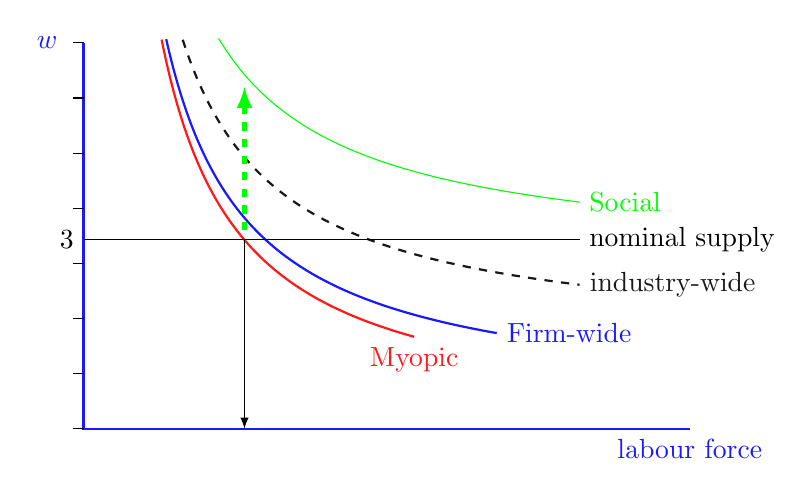
\begin{tikzpicture}[scale=.7]
%\def\bndmax{5}        %https://tex.stackexchange.com/questions/68462/filling-a-complex-region-with-tikz
%\def\bndmin{0.2}
\def \Y {7}  % height of y axis pecent
\def \W {15}  % length  of x axis
\def \Wbar {3} % jmeam wealth
\def \omega {3}
\def \A {1}  %was .5
\def \B {.5}

\draw [thick, color=blue!90] (0,\Y)node[left=.2cm]{$w$} -- (0,0)--(\W-4,0)node[below]{labour force};  
 \foreach \yi in {0,...,\Y} \draw (0,\yi)--(-.2,\yi)node[left]{};
 
\tikzset{func/.style={thick,  color=blue!90}}
% \draw[ func, domain=.2:\W-6] plot [samples=200] (\x, 2*\x^.5)node[below=.1, right]{SUPPLY};

\tikzset{func/.style={  color=green}}	
\draw[func, domain=2.45:\W-6] plot [samples=200] (\x, 10/\x+3)node[above=.1, right]{Social};

\tikzset{func/.style={thick, dashed, color=black!90}}	
\draw[func,domain=1.8:\W-6] plot [samples=200] (\x, 10/\x+1.5)node[ right]{industry-wide };

\tikzset{func/.style={thick, color=blue!90}}	
\draw[func,domain=1.5:\W-7.5] plot [samples=200] (\x, 10/\x+.4)node[below=.05, right]{Firm-wide};

\tikzset{func/.style={thick,color=red!90}}	
\draw[func,domain=8.5/6:\W-9] plot [samples=200] (\x, 10/\x)node[below]{Myopic};

\draw[](0,3.425)node[left]{$\omega$}--(9,3.425)node[right]{nominal supply };
\draw[thin,latex-](2.92,0)--(2.92,3.425); %a vertical labour supply
\draw[ultra thick,dashed, green,-latex](2.92,3.6)--(2.92,6.2);
%\draw [blue,  thick](13, 8.3)--(15,8.3)node [right, black] {\small A=\ 1,\ B=0.5};
%\draw [green, thick](13, 7.6)--(15,7.6)node [right, black] {\small A=.8, B=0.8};

%\node at (5,-1.5){Resulting in  profits, expansion, and/or entry: the city grows};
 \end{tikzpicture}
  \caption{Multiple marginal products}
    \label{fig-Marginal-products}
\end{figure}



Figure~\ref{fig-Marginal-products} illustrates the problem. We can  make a distinction between the myopic marginal productivity curve observed by at the shop floor level and  the firm-wide effect of adding a worker. The red curve labeled ``Myopic'' represents the declining direct marginal productivity of labour as in might be observed by a shop manager, who could report how much more output one with one worker one lathe would produce. The blue line above it labeled ``Firm-wide'' represents the actual effect on firm productivity that arises because the new worker makes other workers in the firm more productive. This addition to output would be observable for managers reviewing the firm's performance over time. ' 

We can go on to consider the slower and distributed effect on closely related firms, which would raise any estimate of marginal product.  If there are 10 other firms and a new worker  has a small spillover effect  $\epsilon$ on each,  the spillovers raise the industry  marginal product  by $10\epsilon$. Each of the  10 other firms  enjoys  an additional $10\epsilon$ gain in the marginal product of their workers. This should lead to additional hiring by other firms.

Finally, expanding our view another step, we notice that if each of the  10 other firms hires one worker who produces an additional  $10\epsilon$ gain in output for all firms, the total spillover effect would rise by $100\epsilon$. The social marginal product of a single hire is indicated by the green line. 



\section{Distribution of rents}
Rents go to landowners, with a share taken for maintenance and taxes.
Rents may also be taxed, could be shared between multiple owners, etc.
 %\note{REPHRASE? rent is  extracted from the coalition of capital and workers.} % Rents may also be taxed, could be shared between multiple owners, etc. 
%The rents are captured by landowners.  The capture of rents by landowners is common buy not necessary. 
In principle the gains from urban productivity and amenity can be allocated as social wealth through shared ownership, as is often done on a small scale with cooperatives and land trusts, distributed to all citizens through something like a social wealth fund, or captured in taxes or fees as Henry George suggested. 
%The rents would otherwise go to labour and capital.





\subsection{Urban Savings - Contributions?}
THIS IS A CONTRIBUTION, BUT ALSO A DISCUSSION OF ONE WAY THIS WORK COULD BE EXTENDED, MIXED WITH A BIT OF MODEL DESCRIPTION

Conventional growth models specify a savings/investment mechanism at the national level. To our knowledge, this has not been done for the city level. We require  savings at two levels. First, since we want to incorporate  households home ownership and a relationship to the financial sector through mortgages, We specify a savings rate out of the spending we have isolated in the `subsistence wage' This means that both urban and rural workers accumulate savings, that savings are age-dependent, making the size of mortgage available also age dependent. 

Homeowners in addition have equity $E=P-M$ in their homes.  ({\color{red}Should newcomers also have equity? or is it built into the savings. Clarify this.} 

A second level of saving is the  investment in capital out of the city surplus. Even raising this question puts us into terra incognita. There are many  channels through which surplus flows into productive investment in the urban contest. One is through public investment in infrastructure. We have discussed how falling transportation costs increase surplus generation. Investments like this are made slowly and take effect over time periods much longer than our model is concerned with.  We can set a property tax rate   that we will assume is sufficient to maintain the stock of infrastructure.

Public and private investment in human capital is largely urban as well, but as with infrastructure, investment and response take effect over time periods much longer than our model is concerned with. 

Private sector innovation in technology, marketing, or products draws on local saving less but still significantly on local savings. We have little in the way of theory or empirical research on this channel. Lags between investment and any rise in the urban wage premium are almost certainly long and variable. 

We deal with this issue by linking local capital ownership with the scale factor. It is known that local ownership is associated with local investment. We will assume that local capital ownership, which consists in part of local ownership of the housing stock, can be proxied by homeowner equity as a share of local. 

\subsubsection{savings and retirement behaviour}
Agents fund their retirement from savings, as well as returns on their home if they have one to sell. Savings may be invested in a pension fund, or in local property,  depending on expected risks and returns. In the real world, financial institution manages most pensions, investing in the market or in property.  All this institutional structure is probably most easily handled by implementing a savings account for each agent. We are not interested in the detailed investment behavour for the financial sector.% either in the stock market, or in pensions.

%Institutional and individual investors can access debt. %

also consider a case where outside money can come under institutional management, not just local retirement savings. A parameter controls the inflow of additional money beyond local investment in the pension fund. 



\subsection{Taxes, municipal government, public goods, and productivity,}
This is a major issue with considerable development in the economics literature. Property taxes reduce the net locational value that flows to an individual owner but provides services and wages that make the city attractive. 

(create a regime where particular groups have an advantage)

Localized tax advantages can move a share of financialised investment into private consolidation of land.
including the structure of taxes for investment properties, institutional investors, individuals, etc.




\section{TO  METHODOLOGY?: Distribution}% not the right word
ABMs can be run multiple times to produce distributions of expected outcomes, which makes them valuable in planning exercises. They also do not require that we use a representative agent to make them tractable. Our model is intended to be elaborated  for such use. 

extensions
what it is
why it would be great to model
why it doesn't matter for our core results

\section{A possible typology of models and experiments}
While there  are very many variations on the basic urban model and many potential experiments with each model there are only a few of immediate interest if the goal is to text the ``resilience'' of equilibria.

These models may exhibit irreversibilities in variables such as distribution, homelessness, city form, and class structure. 

The basic strategy for examining the system resilience is to shock a model (experiment) and then see if diagnostic variables recover. (This needs more precise expression.)

The first task is to select a subset of models an experiments that are of particular interests with respect to.

The second is to construct a model that allows those case to be examined. Ideally the model would be easily adapted to other experiments.

The following is a an attempt to develop a typology with a clear progressive structure.

Feedback - wealth allows upgrading. This advantages the rich. Maybe this 

\subsection{Models}
\begin{enumerate}
\item \textbf{A: The basic model}

The workhorse of urban economics is the circular city model. Some feature of the central place generates rents. It may be that it is the only employment centre. It may be economies of scale to a single activity or synergies arising from various externalities\footnote{We are interested in agglomeration economies. The wage  structure would then be related to the population or industry  structure. Externalities driving agglomeration may be classified  into two types, the  or so-called ``Marshalian''  and ``Jacobs'' externalities.}. 

In the simplest model, the central place pays a uniform wage, $w$ to all employees, who have identical preferences and transportation costs. $w$ is an attribute of individual residents. Residents  purchase or rent equal quantities of land at differing locations $l$ for identical housing.  

There are transportation costs $T$ that depend on distance from the  central place, so land close to the central place is more attractive than land farther from the central place.  

The equilibrium concept is that a market with identical individuals with identical incomes and transportation costs will result in identical utilities. The result is that land rent must decline with distance from the central place to offset rising transportation cost. 

The size of the city is determined by population and lot size. Income and transportation costs will interact with lot size. The basic model can be initialized by matching the number of properties to the size of the population. 

If population exceeds the number of properties there are three margins to consider
	\begin{enumerate}
		\item The land supply can increase. There may be a conversion cost
		\item The land per-capita may decrease. This is not simple in a city with land-use regulations, zoning, and fixed capital in homes. A conversion process has to be defined
		\item A homeless population can emerge. 
	\end{enumerate}

It is convenient in this model to use a \gls{Cobb-Douglas} utility function that has the property that a fixed fraction of income is spent on housing.  We can start with the assumption that earnings are fixed for the lifetime at the one-period wage, $w$. Then total spending on housing is $\beta Y, \beta <1$ and $ Y=w$. Let the transportation cost for a specific location $l$ be $T(l)$. The  equilibrium price at that location will be $P(l)= \beta Y-T(l)$.

It is convenient but not necessary to assume that land outside of the residential limit is costless. It is common to assume a fixed price for agricultural land. 

There is no fixed boundary and the size of the city is determined by the utility that can be achieved in competing regions of competing

\item \textbf{Y: The basic model with Income Differences}
This will result in segregation by neighbourhood depending on income. 

Income can be purely earning, which requires a distribution of $w$ across agents. Income  might include investment income, which  a private rate of return and a distribution of assets across agents. \footnote{A more subtle model could allow individual wages to be linked to the agglomeration of other workers - say engineers. we can imagine a city that has centres of agglomeration by profession or by complementarity. Depending on the production function, this should emerge endogenously.}
\footnote{Sufficient investment income could lead individuals to locate in cheap properties at the edge of the city.  Income might also be invested in property affecting the quality of a unit. This would require incorporating unit quality in the attribute list for each property, and introducing a quality preference  in the attribute s of residents.}

\item \textbf{L: The basic model with Locational Preferences}
This will result in segregation by neighbourhood depending on preferences.

One version would be include distance to the edge of the city as an amenity in the utility function. Another would be to locate amenities within the city. These would lead to higher prices near amenities.

A natural variant would be to have earning depend on location. If there were several locations  a polycentric city would emerge.

\item \textbf{T: The basic model with varied transportation cost }
This will result in segregation by neighbourhood depending on income and Transportation costs. Experiments include cars for the rich and  transit. 

Diagnostics include change in total transportation cost and differential welfare effects.

\item \textbf{R: The basic model with a rent-own choice}
This may result in the emergence of classes. Agents must have the capacity to borrow to purchase. Attributes of the agents and must now include  net assets,  an available interest rate, and a permissible mortgage.

We imagine a banker setting the mortgage rates and size. This can be done at the beginning of each period for each agent. 

With no income differential we expect equal utiliites

\item \textbf{YR: The basic model with earnings (Y) differences and a rent-own choice}
This model is very likely to generate diverging classes as income differentials permit some to capture land rents from others. This is highly likely if borrowing costs decline with income and asset ownership.

\item \textbf{L: The basic model with variable lot size}
This is achieved by making lot size a choice variable for households, in which case we will get a trade off between transportation cost and lot size and distance. Results for this model are known. Density  falls with distance from the centre. 

\item \textbf{YL: The basic model with earnings (Y) differences and variable lot size}
The wealthy choose larger homes and lots farther form the centre

\item \textbf{S: The basic model with constant lot size and variable density}
This is achieved by allowing stacking of housing units. Results for this model are not known. This introduces a step change in housing form, and emphasizes unit size.

This model should produce some interesting spatial patterns, especially if couples with the possibility of secondary central places.

\item \textbf{YS: The basic model with earnings (Y) differences, constant lot size and variable density}

This model should produce some interesting spatial patterns, especially if couples with the possibility of secondary central places.

\item \textbf{IR: The basic model with outside investors and rent-own}

\item \textbf{IYR: The basic model with outside investors, earnings differentials and rent-own choice} This model is of interest if borrowing costs decline with income and asset ownership.
\end{enumerate}
\subsection{Experiments}
There are various experiments of interest. You will have to pick key ones. It is not necessary to do all of them in every model. 

	\begin{enumerate}
		\item increase population
		\item increase wage
		\item add hard boundary (limit land)
		\item Introduce differential incomes
		\item Introduce differential access to capital
	\end{enumerate}

% \newcommand{\cred}{\cellcolor{red!30}}
% \begin{table}[htp]
% \caption{Potential experiments: \textbf{Pick some}}
% \begin{center}
% \begin{tabular}{|c|c|c|c|c|c|}\hline

%   &\multicolumn{5}{c|} {experiments}\\ \cline{2-6}
% Model  &1 &2  & 4 &4  & \\ \hline
%  A& \cred& \cred  &  \cred & \cred  & \cred  \\
%  Y& \cred   & \cred   & \cred   &\cred    &\cred   \\
%  T & \cred   & \cred   & \cred   &\cred    &\cred   \\
%  R & etc &  &  &  & \\
%  L &  &  &  &  & \\
%  S&  &  &  &  & \\
%  I &  &  &  &  & \\
%  YR &  &  &  &  & \\
%  IR &  &  &  &  & \\
%   IYR&  &  &  &  & \\\hline
% \end{tabular}
% \end{center}
% \label{default}
% \end{table}%

\chapter{Future work to SORT}
model development (experiments and extensions)
interventions
theoretical development
% The urban production sector pays a wage premium $w$
%This is a convenient simplification, not a necessary feature of the model. 

The rental value of land shapes the city spatially.  

\section{Experiments with this model}
Lots of simple extensions e.g. 2 cities with immigration, differentiated labour, products, market power, neighbourhood effects (see extensions map/typology), we focus on those elements central to seeing the structure of the resilience dynamics of the wealth/housing effect. Consider adding density, to look at how it interacts with agglomeration effects. (integrating with transportation effects is very neat)

\subsection{Initial state}
Basic experiments has all homes owner occupied to start. Other initial tenure mixtures are easily modelled. WHY WE MIGHT WANT TO

The basic model can be initialized by matching the number of properties to the size of the population. 

In the simplest version, firms concentrate at the city centre. Workers are spread over space and pay transportation costs to commute.

The size of the city is determined by population and lot size. Income and transportation costs will interact with lot size. 

\subsection{Parameter values}

\subsection{Analysis methods}
mapping of regimes

\subsection{Data}
incorporation of local data more carefully

\section{Extensions to the model}
The simple circular city can be extended to to produce other forms, including polycentric cities and hierarchies of cities at the cost of additional computational complexity. The simple case we examine will allows us to focus on the general, and neglected, distributional features of this class of models.

\subsection{Lags and adjustment processes}
The details of the adjustment process and the system lags are selected primarily for convenience in simulations. Real-time lags are important and complex, we explore some sensitivity results, but can explore more. 

We model a fairly short lag although in reality lags are long and variable. 

\subsection{Labour adjustment costs}

in the agent model, employees are simply laid off and seek work, so there is unemployment, but there are not \glspl{labour adjustment cost} for firms.

\subsection{Agglomeration effects, and returns to scale}
The case where there are increasing returns at the city level introduces interesting dynamics, explored in appendix CITE % 'furthur discussion' appendix.

We incorporate agglomeration effects using a Cobb Douglas formulation. This allows us to focus on the results of agglomeration in the urban system, rather than specifying the system of firms that transmit the effect. 
There are a number of other ways to study the aglomeration process in more or less explicit ways.

MOVE TO PARAMETER VALUE DISCUSSION?
The strength of the agglomeration is given by $\gamma$, thus for $\gamma=0$ there are not agglomeration effects. APPENDIX?
By definition, with one person, the agglomeration effect has no influence, $\Lambda(1)=1$,  as in the \gls{Cobb-Douglas}, and empirical urban scaling results tell us that agglomeration increases with population, following a power law distribution, so we know %$\die
FIX EQN ERROR die ${\Lambda}{n}>0$. 
%%%%%%%%%. ***WHY
If $\beta=1-\alpha$, this is a \gls{constant returns to scale} production function. Without agglomeration effects, $T(n)=1$,  Then  \textbf{$\mathbf{L(n) = T(n) n}$}  WHAT IS T, WHAT IS THIS TELLING US?
Without agglomeration effects, $\Lambda(n)=1$,  Then  \textbf{$\mathbf{L(n) = T(n) n}$} 


\subsection{Returns to scale and firm under-investment}
Each firm has \gls{decreasing returns to scale}, which means each new worker increases output by less than the previous worker did.
RETURNS TO FIRM CAN BE DECLINING WHILE RETURNS TO CITY INCREASING, THEN FIRM UNDER INVESTS
explore this in the model, see Equation \ref{Eqn:Prod1}.

\begin{equation}
Y=K_i^{\alpha }(\Lambda(n)n_i)^{\beta }.
% \label{Eqn:Prod1}
\end{equation}

MOVE DISCUSSION HERE FOR NOW

\subsection{Heterogeneous agents}
In the simplest model, the central place pays a uniform wage premium, $w$ to all employees, who have identical preferences and transportation costs. 
The wage $w$ is an attribute of individual residents.  
It is straightforward to vary i and to vary preferences. 

relax assumptions and look at how the interaction between the production of social wealth in cities interacts with housing and the extraction of rent to drive patterns in a richer model with heterogenous agents interacting over space and time. 

- wages, skill sets

\subsection{Forward looking agents}
There are reasons to expect the results obtained with  forward-looking agents to differ substantially from those obtained with a model featuring myopic agents.\footnote{For example, Lecca et al. *** \cite{LOST-Lecca-et-al-2013}  used a stylized computational macroeconomic model applicable to a regional context to demonstrate that the assumption of myopic vs forward-looking agents yields differences in the dynamics generated by a shock perturbing the initial steady state, even though the alternative paths lead to the same long-run equilibrium.} 

\subsection{Rental bidding process}
 "Just as with prices, there is an economically \gls{warranted rent} which may differ from the \gls{market rent}. Individuals make their investment decisions on their own expectations rents. the bidding process on rental properties is abstracted in the base model. Instead of modelling the process explicitly, we make the assumption that the warranted rent is the market rent, $\mathcal{R}_W = \mathcal{R}_M$." .. could implement

\subsection{Amenity}
Notation for amenity.
There may be a band surrounding the city or persons who do not commute but enjoy urban consumption amenities. 
based on location etc

\subsection{Preferences}
A utility function/algorithm specifies agents preferences over the attributes that matter. - algorithmic continuous. lexicographic- any traits. 

\subsection{Unemployment and labour adjustment costs}
There is no unemployment. there are no labour adjustment costs for firms. ***INTERESTING TO THINK ABOUT  
when people would stop working with

 falls to subsistence wage -
 too much rent, I guess they leave, they can always move somewhere

\subsection{Moving costs}
     If there are moving costs, people can be trapped in a bad situation, incurring debt, and it can still be not worthwhile to move

\subsection{Mobility}
We could look at mobility in a more sophisticated way..
Agents enter the urban market two ways. If wages rise, agents just outside the city may become commuters. This increases population. 

When homeowners in the city retire they sell their home and move to the country. This allows them  to enjoy the capital value of their home.  They either sell their home or rent it to a new occupant. 

When  tenants in the city retire they would move to the country to enjoy lower rents. This has no effect on population. It is simplest, therefore to treat tenants as permanent residents unless we want the tenant's retirement to trigger an event like a rent increase or a decision by the owner to sell the property.

\subsection{Transportation costs}
Wage and transportation cost determine the radius of the circular city, which determines the size of the labour force which affects urban productivity. The cost of travel is therefore an important variable in the development of urban productivity. 

the transportation cost/distance relationship appears to be non-linear in many cases. While the linear model connects with the established literature, we likely want to explore the implications of more empirically grounded curve (e.g. \cite{bertaudSpatialDistributionPopulation2003}).

\subsection{Multiple firms and production structure}
The scaling result at the level of the city allows us to incorporate the effect of agglomeration in a standard \gls{circular city} model in a simple way. 

We could also explicitly model labour markets and competing firms. 

Explicitly modelling labour markets with multiple firms is a natural way to specify the model more completely, see Appendix \ref{appendix-future-work},  but it would require introducing many ancillary assumptions and selecting among alternative models of agglomeration, when when we want to focus on distributional and growth-affecting features of the system.

For simplicity, assume firms produce a variety of perfectly substitutable commodities which are exported and locally consumed at a fixed price in a large market. 
***  Increasing product variety may produce a consumption agglomeration economies as in \cite{fujitaSpatialEconomyCities1999}.

\subsection{Market power and interchangeable goods - local markets etc}
MAKE A FOOTNOTE ON MARKET POWER AND INTERCHANGIBLE GOODS??
No externalities imperfect information etc.. ensure efficiency but aren't needed, all you need is price taking for individuals to only pay attention to their own costs and their own benefits. 

\gls{externalities}, \gls{imperfect information}, \gls{monopsony}, \gls{duopoly}, \gls{monopoly}

competitive markets many sellers, many buyers, monopoly single seller, monopsony - single buyer, intermediate cases - monopolistic competition - with some market power but not complete - duopoly- some inefficiency depending on the behavioural model because in the duopoly case they may be able to take advantage of the behaviour of buyers.

Start with perfect competition, then introduce monopolistic competition is most likely.. but it's more difficult to handle. e.g. with brand names, people have some preference for some feature of your particular good so you can price it higher even though you may loose some marginal people. Firms compete on brand name and reputation, not the pure cost effect.

In the spatial economy, goods are deferentially interchangeable. Put them on a line and firms pick a place along they line. Firms are in competition but are competing on a line-.. spatial model moved over to characteristic space..---looking at this would involve overlaying another space - the characteristic space on the physical space. .. There are also local places with local grocery stores. Polycentric stores have effectively monopolistic competition in real space. - like a named cafe downtown has the same.

\subsection{Sectors}
..


\subsection{Incomes}
In the model receive the\gls{urban wage}, which is the subsistence wage plus the urban wage premium $\psi + w$.

They may get different incomes because of firm, sector or individual increases, or particularities of the 
hiring/negotiation/wadge adjustment process, path dependency, stochasticity, etc. 
All of these factors could be explored formally in the model. %ref{rockefeller}


POOR STRUCTURALLY DISADVANTAGED HOWEVER RICH WE GET
these are averages-- some are structurally below average so some are always behind simply because of the structure of the rents claimed.. that's built in FUTURE WORK- DIFFERENT INCOMES GETS YOU THAT. 



\subsection{Hiring process and unemployment} \label{rockefeller}
 In our model, non-urban landowners are those who live too far from the urban job center to justify commuting.  Agents join the urban market by adding their names to the firm's list of job applicants when the rent on the marginal unit of land exceeds the transportation cost. 

adjustment speeds..
 
i(did extended modelling in the Rockefeller social innovation lab)- barriers of employment for young people seeking work
- prison records, transportation, family responsibility, bias, educational attainment, expectations of success, neighbourhood factors etc.
Could explore that kind of structure in this model

\subsection{Demographics}
Could build a population model suited to particualr data sets %\ref{rockefeller}

\subsection{Skills and individual productivity}
The basic model consideres a non-differentiated workforce. We can add particular skills.
Some agents can be more productive than one another

Agents may move to cities to assemble networks (model as networks)
and learn specialized skills

It can evolve over time so agents can productively over pay to  
-- getting debt/resources at key stages in a persons development to aquire property and skills is important to \gls{wealth trajectories}


\subsection{Sources of agglomeration effects}
Some of the empirically wage difference comes from the dense resources  - location of cities in good places, public investment- libraries - institutions, the network effects
some from the ability of those close to the center to simply claim a larger share of resources
some 
Some of the agglomeration wage may come from people with resources and skills disproportionately choosing cities for their amenity effect. 

We can explore different drivers in the model.


\subsection{TO METHODOLOGY: Rural market and other cities}

 To simplify analysis, we assume that land outside of the residential limit is costless, following th common practice of assuming a fixed price for agricultural land \cite{GET_fixed-price-ag-land}. 

The model is constructed so that there is neither land rent nor capitalist exploitation in the rural economy. 
This special case allows us to examine the distribution of the social surplus generated by agglomeration economies and the effect of financialization.

We could explore this

\section{Interventions: Policy and Agent Strategies}
Extended appropriately, this basic model could be used for planning.

detailed models of interventions typologies of interventions e.g. local currencies, decaying currencies, 

\subsubsection{Teaching}
could use for teaching a sequence for illustration could follow to introduce x ideas - see above. - rent, space, finance treated separately, - tool to think about their relation

productivity centered urban and spatial policy

connects with growth, economic development in real places work

\subsection{Zoning}
zoning - layers interact

\subsection{Taxes}
property taxes reduce the net locational value that flows to an owner but provides services and wages that make the city attractive. 

(create a regime where particular groups have an advantage)

Localized tax advantages can move a share of financilized investment into private consolidation of land.
including structure of taxes for investment properties, institutional investors, individuals, etc.


\subsection{Insurance, risk, and mortgage backing}

Uncertainty is a key variable.

The effects of policy are large. For example in Canada, backing mortgages is the largest fiscal investment at the national level \cite{nemtinFinancializationHousingSocial2021}.

- risks, bubbles, collapse


\subsection{Housing quality, size, subdivision}
Residents  purchase or rent equal quantities of land at differing locations %$l$ 
for identical housing.  DOWN

? More generally, if we were to introduce variations in lot size and housing types  we would want the integral of the worker density function. In our ABM version  of the model we simply count the workers within the commuter shed.

\subsection{Development and Improvements}
The supply of land at any distance from the center is inelastic. 
Its value comes from proximity to the productive urban centre, not from the value of improvements made to the property.

*** Without density, the labour supply increases with the square of the wage.  other forms..

- We have an empirical curve - gives density- simply build in

- We can .. Model a subdivision process-- urban SIM, a collaborator on the missing middle grant. - model of pro-forma and typoloties/ policies makes it possible to follow..

Some nonlinearities e.g. Some may buy land seeking to develop property in the future and let it become run down. 

We could add improvements
 or consolidation, subdivision, and development. 

% Reference sections on development which is different, and the contribution of amenity % Because supply is fixed for urban land, and the landowner has a monopoly claim on rents, the rents that can be depend on wages and amenity rather than the cost of improvements made to the property.
% The source of rents is the free gifts of nature, the coming together of people to create value in cities, and the concentration of public amenity in cities. 




\section{SORT Rough Notes}
what does a speculative over investment.  in housing  do? - hollowed out store front

who carries what risks- banks vs individuals

subdivision and density

multiple cities,
linear cities

differential skills and wages,
work from home

details of typologies, transportation networks, etc

- make it available as a part for other models, use other models in this model


 

\subsection{Implications}
\subsubsection{Agglomeration driven under-investment}
